\documentclass[12pt,a4paper]{article}
\usepackage{cmap} % Makes the PDF copiable. See http://tex.stackexchange.com/a/64198/25761
\usepackage[T1]{fontenc}
\usepackage[brazil]{babel}
\usepackage[utf8]{inputenc}
\usepackage{amsmath}
\usepackage{amsfonts}
\usepackage{amssymb}
\usepackage{amsthm}
\usepackage{textcomp} % \degree
\usepackage{gensymb} % \degree
\usepackage[usenames,svgnames,dvipsnames]{xcolor}
\usepackage{hyperref}
\usepackage{multicol}
\usepackage{graphicx}
\usepackage[margin=2cm]{geometry}

\hypersetup{
    colorlinks = true,
    allcolors = {blue}
}

\newcommand*\sen{\operatorname{sen}}
\newcommand*\dom[1]{\operatorname{Dom}\left(#1\right)}

\newcommand*\R{\mathbb{R}}

\newcommand*\tipo{PROVA III}
\newcommand*\turma{MAT102-02U}
\newcommand*\disciplina{CDI0001}
\newcommand*\eu{Helder G. G. de Lima}
\newcommand*\data{18/11/2015}

\author{\eu}
\title{\tipo - \disciplina}
\date{\data}

\begin{document}
\thispagestyle{empty}
\newgeometry{margin=2cm,bottom=0.5cm}
\begin{center}

\includegraphics[width=9.0cm]{marca}
\noindent\begin{tabular}{l c c r}
  \textbf{\disciplina (\turma)}
& \textbf{\tipo}
& \textbf{\data}
\end{tabular}
\\ Prof. \eu\footnote{
Este é um material de acesso livre distribuído sob os termos da licença \href{https://creativecommons.org/licenses/by-sa/4.0/deed.pt_BR}{Creative Commons BY-SA 4.0}.}
\end{center}

\noindent Nome do(a) aluno(a): \rule{13cm}{0.01cm}

%\section*{Instruções}
\begin{center}\fbox{
\begin{minipage}{14cm}

{\footnotesize
\begin{itemize}
\renewcommand{\theenumi}{\Roman{enumi}}
\item Identifique-se em todas as folhas.
\item Mantenha o celular e os demais equipamentos eletrônicos desligados durante a prova.
\item Justifique cada resposta com cálculos ou argumentos baseados na teoria estudada.
\item Resolva (integralmente) apenas os itens de que precisar para somar 10,0 pontos.
\end{itemize}
}

\end{minipage}
}
\end{center}


%\section*{Questões}

\begin{enumerate}

\item (3,0) Calcule os seguintes limites, utilizando as regras de L'Hôpital quando for apropriado.
\begin{multicols}{3}
\begin{enumerate}
\item $\displaystyle\lim_{x\to\infty} \frac{x}{\sqrt{x^2+1}}$
\item $\displaystyle\lim_{x\to +\infty} \frac{\cos(x)-1+\frac{x^2}{2}}{x^4}$
\item $\displaystyle\lim_{x\to 0^+} x^{1/x}$
\end{enumerate}
\end{multicols}

\item (1,0) Explique o erro (com um exemplo simples que mostre o problema) no seguinte raciocínio: ``Se $f^{\prime\prime}(x_0) > 0$, então $x_0$ é um ponto de mínimo da função $f$''.

\item (3,0) Considere a função \[f(x) = \begin{cases}
e^{-1 / x^2}, & \text{ se } x \neq 0 \\
0, & \text{ se } x=0.
\end{cases}\] Esboçe o gráfico de $f$, explicitando o domínio, simetrias, zeros, intervalos de crescimento e decrescimento, pontos de máximo e mínimo, concavidade, pontos de inflexão, assíntotas e limites que forem relevantes. Não esqueça de justificar suas afirmações!

\item (1,5) Seja $f: \R \to \R$ uma função derivável que tem um ponto de mínimo local em $x_0$. O que se pode concluir sobre a função $g(x) = 1 - f(x)$ no ponto $x_0$? Explique a sua conclusão (dica: inspire-se em algum um exemplo).

\item (2,0) Mostre que de todos os triângulos isósceles (isto é, com dois lados iguais) com um dado perímetro $P > 0$, aquele que tem a maior área é o equilátero (todos os lados iguais).

\item (1,5) Faça um esboço do gráfico de $f$, assumindo que$f: [-4, +\infty) \to \R$ seja uma função derivável cujo gráfico passa por $A=(-4,3)$, e cuja derivada tem o seguinte gráfico:

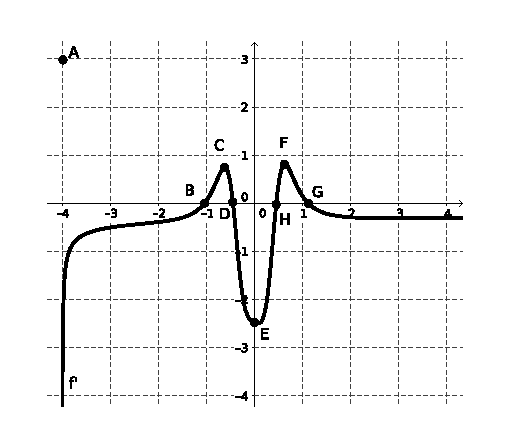
\includegraphics[width=8.0cm]{img/prova-3-mat-grafico-f'}

\end{enumerate}

\newpage
\restoregeometry
\section*{Respostas e observações}
\begin{enumerate}
\item \textit{Calcule os seguintes limites, utilizando as regras de L'Hôpital quando for apropriado.}
\begin{enumerate}
\item $\displaystyle\lim_{x\to\infty} \frac{x}{\sqrt{x^2+1}}$
\[
  \lim_{x\to\infty} \frac{x}{\sqrt{x^2+1}}
%=\lim_{x\to\infty} \frac{\sqrt{x^2}}{\sqrt{x^2+1}}
= \lim_{x\to\infty} \sqrt{\frac{x^2}{x^2+1}}
= \sqrt{ \lim_{x\to\infty} \frac{x^2}{x^2+1}}
= \sqrt{ \lim_{x\to\infty} \frac{2x}{2x+0}}
= \sqrt{1}
= 1
\]

\item $\displaystyle\lim_{x\to +\infty} \frac{\cos(x)-1+\frac{x^2}{2}}{x^4}$
\begin{align*}
  \lim_{x\to +\infty} \frac{\cos(x)-1+\frac{x^2}{2}}{x^4}
& = \lim_{x\to +\infty} \frac{-\sen(x)+x}{4x^3}
= \lim_{x\to +\infty} \frac{1}{12x^2}(-\cos(x)+1)
= 0
\end{align*}
\item $\displaystyle\lim_{x\to 0^+} x^{1/x}$

Como $x^{1/x} = e^{\ln( x^{1/x} )} = e^{ \frac{1}{x} \cdot \ln( x ) }$ e $\lim_{x\to 0^+}\frac{1}{x} \cdot \ln( x ) = -\infty$, tem-se
\[
  \lim_{x\to 0^+} x^{1/x}
= \lim_{u\to -\infty} e^{u}
= 0.
\]

Note que não é possível aplicar L'Hôpital, por não ser um limite do tipo $\frac{ \pm\infty }{ \pm\infty }$ nem $\frac{0}{0}$.
\end{enumerate}

\item \textit{ Explique o erro (com um exemplo simples que mostre o problema) no seguinte raciocínio: ``Se $f^{\prime\prime}(x_0) > 0$, então $x_0$ é um ponto de mínimo da função $f$''. }

Para que $x_0$ seja um ponto de mínimo da função $f$, não basta que a segunda derivada de $f$ seja positiva neste ponto: também é necessário que a primeira derivada seja igual a zero. Por exemplo:
\begin{itemize}
\item Se $f(x) = e^x$, então $f^{\prime\prime}(x) = f^\prime(x) > 0$, para todo $x \in \R$, e no entanto $f$ não possui qualquer ponto de mínimo.
\item Se $g(x) = x^2$, então $g^\prime(x) = 2x$ e $g^{\prime\prime}(x) = 2 > 0$, para todo $x \in \R$, e nem por isso o ponto $x=1$ é um ponto de mínimo da função.
\end{itemize}

\item \textit{ Considere a função \[f(x) = \begin{cases}
e^{-1 / x^2}, & \text{ se } x \neq 0 \\
0, & \text{ se } x=0.
\end{cases}\] Esboçe o gráfico de $f$, explicitando o domínio, simetrias, zeros, intervalos de crescimento e decrescimento, pontos de máximo e mínimo, concavidade, pontos de inflexão, assíntotas e limites que forem relevantes. Não esqueça de justificar suas afirmações!}

Observe que $\dom{f} = \R$ e que $f(x) > 0$ sempre que $x \neq 0$. Além disso, a função é par, pois (para $x \neq 0$) vale
\[
f(-x)
= e^{-1 / (-x)^2}
= e^{-1 / x^2}
= f(x).
\]
Assim, o gráfico de $f$ é simétrico em relação ao eixo vertical. Note que em $x \neq 0$ a função $f$ é contínua (por ser uma composição de funções contínuas) e em $x=0$ tem-se
\[
\lim_{x \to 0} f(x)
= \lim_{x \to 0} e^{-1 / x^2}
= \lim_{u \to -\infty} e^u
= 0
= f(0).
\]
Logo, $\lim_{x \to a} f(x) = f(a) \neq \pm \infty$ em todo ponto $a \in \R$ e não há assíntotas verticais. Por outro lado, tem-se
\[
\lim_{x \to \pm \infty} f(x)
= \lim_{x \to \pm \infty} e^{-1 / x^2}
= \lim_{u \to 0} e^u
= e^0
= 1,
\]
ou seja, $y=1$ é uma assíntota horizontal. Tem-se ainda, para $x \neq 0$, que:
\[
f^\prime(x)
= e^{-x^{-2}} \cdot (2x^{-3})
= 2 x^{-3} e^{-1/x^2}
\]
e portanto $
f^\prime(x) < 0
\Leftrightarrow 2 x^{-3} e^{-1/x^2} < 0
\Leftrightarrow 2 x^{-3} < 0
\Leftrightarrow x < 0$. Isto significa que $f$ é decrescente em $(-\infty, 0)$ e crescente em $(0,+\infty)$, tendo então um ponto de mínimo local em $x = 0$. Como a função exponencial só assume valores positivos, $f(x) > 0 = f(0)$ para todo $x \in \R^*$, e o ponto de mínimo também é um mínimo global.

A concavidade de $f$ fica determinada pelo sinal de $f^{\prime\prime}$, que para $x \neq 0$ é dada por:
\begin{align*}
f^{\prime\prime}(x)
& = 2(x^{-3} \cdot e^{-x^{-2}})^\prime \\
& = 2( -3 x^{-4} \cdot e^{-x^{-2}}
  + x^{-3} \cdot 2 x^{-3} e^{-x^{-2}} ) \\
& = 2 x^{-4} e^{-x^{-2}} (-3 + 2 x^{-2}) \\
& = \frac{ 2 e^{-1/x^2} (-3 + 2/x^2) }{ x^{4} }.
\end{align*}
Consequentemente, $f^{\prime\prime}(x) > 0 \Leftrightarrow -3 + 2/x^{2} > 0 \Leftrightarrow 1/x^{2} > 3/2 \Leftrightarrow x^2 < 2/3$, o que implica que a $f$ tem concavidade para cima em $\left( \frac{-\sqrt{2}}{3},\frac{\sqrt{2}}{3}\right)$, e para baixo nos intervalos $\left( -\infty, \frac{-\sqrt{2}}{3} \right)$ e $\left( \frac{\sqrt{2}}{3}, +\infty\right)$. Devido a estas mudanças de concavidade, há dois pontos de inflexão, em $x = \pm\frac{\sqrt{2}}{3}$.

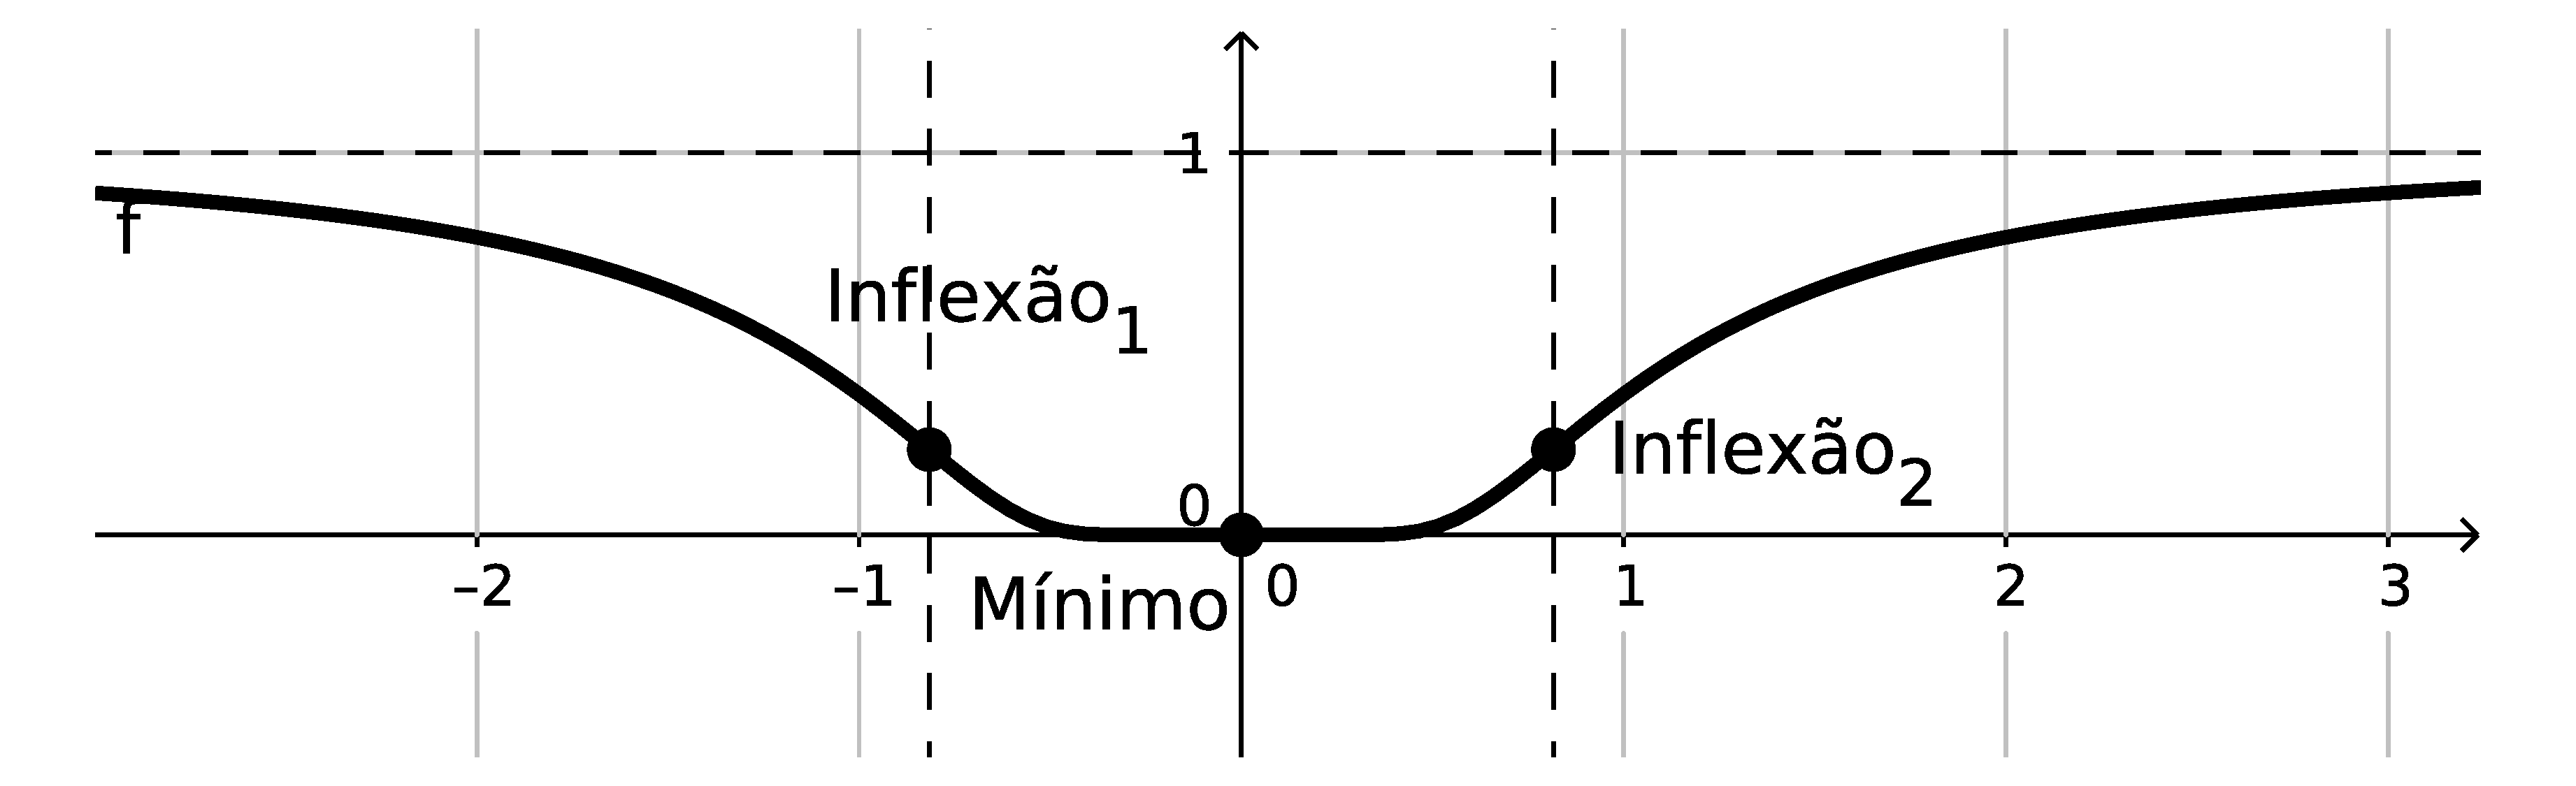
\includegraphics[width=15cm]{img/prova-3-mat-3-grafico-f}

\item \textit{ Seja $f: \R \to \R$ uma função derivável que tem um ponto de mínimo local em $x_0$. O que se pode concluir sobre a função $g(x) = 1 - f(x)$ no ponto $x_0$? Explique a sua conclusão (dica: inspire-se em algum um exemplo).}

Tomando como exemplo a função $f(x) = x^2$, tem-se um mínimo local em $x_0 = 0$. De fato, $f^\prime(x) = 2x$ e $f^\prime(0) = 2 \cdot 0 = 0$ e $f^{\prime \prime}(x) = 2 > 0$. Por outro lado, se $g(x) = 1-f(x) = 1-x^2$ então $g^\prime(x) = -2x$ e $g^{\prime\prime}(x) = -2$, o que implica que $x_0 = 0$ também é um ponto crítico de $g$, mas desta vez, ele é um ponto de máximo.

Note que para qualquer outra função $f$ nas condições acima, continuaria sendo verdade que $f^\prime(x_0) = 0$, e como $g^\prime(x) = (1-f(x))^\prime = -f^\prime(x)$, o ponto $x_0$ também seria um ponto crítico de $g$. Além disso, sendo $x_0$ um ponto de mínimo de $f$, isto é, sendo $f(x) > f(x_0)$ nas vizinhanças de $x_0$, a função $g$ teria um ponto de máximo em $x_0$, pois
\[
f(x) > f(x_0)
\Rightarrow -f(x) < -f(x_0)
\Rightarrow g(x) = 1-f(x) < 1 - f(x_0) < g(x_0).
\]

\item \textit{ Mostre que de todos os triângulos isósceles (isto é, com dois lados iguais) com um dado perímetro $P > 0$, aquele que tem a maior área é o equilátero (todos os lados iguais). }

Em um triângulo isósceles cuja base mede $x>0$ e as demais arestas medem $y>0$, o perímetro é $P=x+2y$, ou seja, $x = P-2y$. Já a altura $h$ relativa à base pode ser obtida observando que no triângulo retângulo obtido ao ligar o ponto médio da base ao vértice oposto tem-se $y^2 = \left( \frac{x}{2} \right)^2 + h^2$. Disto segue que
\[
h = \sqrt{ y^2 - \left( \frac{x}{2} \right)^2 }
  = \frac{1}{2} \sqrt{ 4y^2 - (P-2y)^2}
  = \frac{1}{2} \sqrt{ 4y^2 - (P^2 - 4Py+4y^2)}
  = \frac{1}{2} \sqrt{ 4Py - P^2}.
\]
Assim, a área do triângulo é dada em função de $y$ por
\[
A
= A(y)
= \frac{x \cdot \frac{1}{2} \sqrt{ 4Py - P^2}}{2}
= \frac{P-2y}{4} \sqrt{ 4Py - P^2}.
\]
Os pontos críticos desta função são obtidos a partir da primeira derivada, que é:
\begin{align*}
A^\prime(y)
& = \left[ \frac{P-2y}{4} \sqrt{ 4Py - P^2} \right]^\prime
  = -\frac{1}{2} \sqrt{ 4Py - P^2}
    + \frac{P-2y}{4} \frac{4P}{2 \sqrt{ 4Py - P^2} } \\
& = -\frac{ 4Py - P^2 }{2\sqrt{ 4Py - P^2}}
    + \frac{P^2-2Py}{2\sqrt{ 4Py - P^2} }
  = \frac{-6Py + 2P^2}{2\sqrt{ 4Py - P^2} }
  = \frac{-3Py + P^2}{\sqrt{ 4Py - P^2} }.
\end{align*}
Tem-se $A^\prime(y) = 0$ se, e somente se, $-3Py + P^2 = 0$, isto é, $3Py= P^2$, ou seja, $y = P/3$. Neste caso, $x = P-2y = P-2(P/3) = P/3 = y$ e o triângulo é equilátero. Além disso, como $-3Py + P^2 > 0 \Leftrightarrow P^2 > 3Py \Leftrightarrow y < P/3$, este é um ponto de máximo para a função área.

\item \textit{ Faça um esboço do gráfico de $f$, assumindo que$f: [-4, +\infty) \to \R$ seja uma função derivável cujo gráfico passa por $A=(-4,3)$, e cuja derivada tem o seguinte gráfico:}

\begin{minipage}[]{0.57\linewidth}
O gráfico de $f^\prime$ indica que:
\begin{itemize}
\item $f$ é decrescente de $A$ até $B$, de $D$ até $H$ e de $G$ em diante, pois $f^\prime$ é negativa nestes intervalos
\item $f$ é crescente de $B$ até $D$ e de $H$ até $G$, pois $f^\prime$ é positiva nestes intervalos
\item $f$ tem concavidade para cima de $A$ até $C$ e de $E$ até $F$, pois $f^\prime$ é crescente nestes intervalos
\item $f$ tem concavidade para baixo de $C$ até $E$ e de $F$ em diante, já que $f^\prime$ é decrescente nestes intervalos.
\item $C$, $E$ e $F$ são pontos de inflexão, devido às mudanças de concavidade nestes pontos
\item $B$ e $H$ são mínimos locais de $f$, devido à mudança de decrescente para crescente nestes pontos
\item $D$ e $G$ são máximos locais de $f$, devido à mudança de crescente para decrescente nestes pontos
\end{itemize}
\end{minipage}
\begin{minipage}[]{0.42\linewidth}
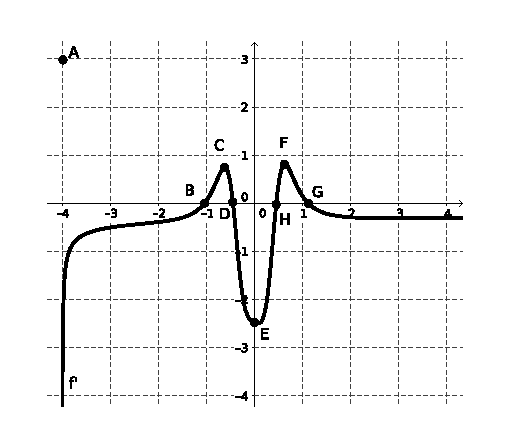
\includegraphics[width=6.7cm]{img/prova-3-mat-grafico-f'}

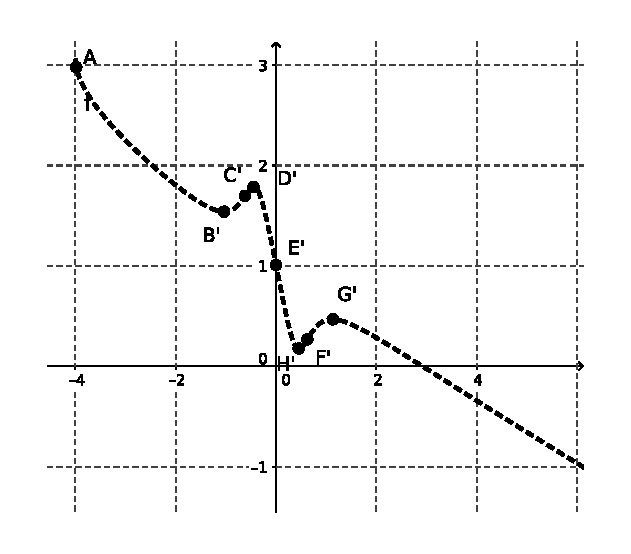
\includegraphics[width=6.7cm]{img/prova-3-mat-grafico-f}
\end{minipage}
\end{enumerate}

\end{document}
